\subsection{OpenCL}

\subsubsection{Standarized framework for heterogeneous systems}

OpenCL is a parallel programming framework designed to fit heterogeneous systems where one can expect a range of different computing architechures. One example of a program on a heterogeneous system would be a program where some parts of the computations and setups are done on the CPU and the rest on the GPU. OpenCL also supports parallel programming for homogeneous systems. In a case where one has a multi-core CPU, OpenCL could be used to in such way to have one thread control the state of the program while the rest of the threads performs a computation of some sort and later sync with the main thread.
\newline

OpenCL is standarized by the Khronos Group, the same group in charge of well known OpenGL standarization. The group consits of people from many different companies in the industry such as AMD, nVIDIA, intel, Apple, Samsung. This is seen as a positive thing as they all decide the direction the group is taking. It also makes sure the framework compatible for different system and platforms. One of the goals of OpenCL is to be as flexible as possible.
\newline

\subsubsection{The OpenCL C language}
OpenCL can be used in any parallel environent as long as the OpenCL compiler and runtime library is implemented. This means, when writing the parallel code, a software developer do not have have care about operating system, processors and memory types. The OpenCL C language is very similar to the regular C language. It is focused around computations and some features are added on top of the C language to simplfy things, like SIMD vector operations and multiple memory hierarhies. Other features, such as printing, have been removed as they are not as useful in computing and hard to implement on all platforms. The program calling the OpenCL code can be written in either C or C++ as it will be using the OpenCL runtime library. 
\newline

The notion of host is often used in standard and offical OpenCL literature. The host refers to the environment where the OpenCL code is called from (not executed). This is the CPU in almost all of the cases. An OpenCL device is the environment where the OpenCL is executed. This can be the GPU, DSP, CELL/B.E, CPU are some examples of OpenCL devices that often contain a lot of small compute units each. The memory associated with these processors are also included in the defintion of an OpenCL device. The OpenCL code executed on a device is called \emph{kernel}.
\newline

\subsubsection{Memory Hierarchy}

Similar to the CUDA architechure, OpenCL also has a memory hierarchy. The OpenCL standard only specifices the access levels of the different memory spaces and there may be important performance details that are different on different hardware implementations. While it makes it possible to optimize the code for a certain hardware or vendor, it makes it harder to generalize and write programs with high performance accross different devices. 

\begin{figure}[ht!]
\centering
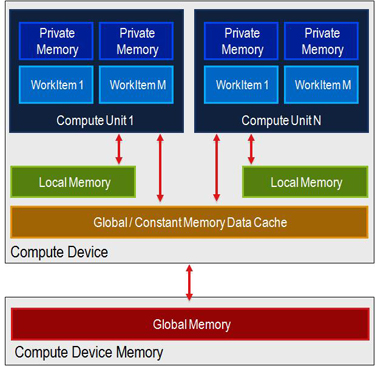
\includegraphics[width=70mm]{img/mem-cl.jpg}
\caption{OpenCL memory hierarchy.}
\label{cl-mem}
\end{figure}

\begin{itemize}
\item{{\bf Global Memory} - The global memory has the larget capacity and can be used by all work items. It is considered of being the slowest memory subsystem. The best performance is achieved when streaming contiguous memory addresses or patterns that can explore the full bandwidth (similar to the coalesced memory reads in CUDA). }
\item{{\bf Private Memory} - The memory used in a single work items. Can not be shared between work items. Similar to registers in GPU multiprocessors or CPU cores. The private memory is allocated and partioned at compile time. There is no maximum private memory size defined  in the OpenCL specification. Using too much private memory can lead to a slowdown since OpenCL will user slower memory spaces once the private memory is full.}
\item{{\bf Local Memory} - Local memory can be shared between work items in a work group, similar to the shared memory in the CUDA architechure. Local memory is used when data from global memory is needed and one wants to reduce the global memory reads within a work group.}
\item{{\bf Constant Memory} - Constant memory is implemented differently on certain deviced. For example, on NVIDIA GPU cards, the constant memory is located at region good for broadcasting. On ATI GPU cards, the constant memory is part of the global memory but with optimized broadcasting.}
\end{itemize}

\subsubsection{Work Groups}

Kernels are being executed over a 1D, 2D, 3D grid or NDRange. The kernel is then executed in parallel where each kernel instance is called work item. Work items are divided in work groups of the global grid. The developer can explicity set the size of the work group or let it be decided at runtime.

\renewcommand{\lstlistingname}{Code}
\begin{lstlisting}[caption= Example of vector addition in OpenCL, label=cl1]
__kernel void VectorAddition( __global float * A,
                              __global float * B,
                              __global float * C,
                              int width)
{ 
    const int x = get_global_id(0); 
    const int y = get_global_id(1); 
    const int idx = x + y * width;
    C[idx] = A[idx] + B[idx];
}
\end{lstlisting}

Code \ref{cl1} shows an example of a simple vector addition. Keyword \texttt{\_\_kernel} tells the compiler it is a OpenCL kernel and \texttt{\_\_global} specifices a pointer to the global memory space. Inside the kernel, the function \texttt{get\_global\_id} is used to find the horizontal and vertical id of the work item (this only works if the kernels are executed with a two dimensional work size).
